\documentclass[border=8pt]{standalone}
\usepackage{amsmath,amssymb}
\usepackage[scaled]{helvet}                 % Arial-equivalent sans (OUP: sans-serif, prefer Arial)
\renewcommand{\familydefault}{\sfdefault}   % sans is the DEFAULT; text sans, math stays serif
\usepackage{xcolor}
\usepackage{tikz}
\usetikzlibrary{arrows.meta,positioning,calc,fit,backgrounds,shapes.geometric}

% ---- macros (mirror supplement_engine_math.tex) ----
\newcommand{\BetaBin}{\mathrm{BetaBin}}

% ---- palette ----
\definecolor{stateblue}{HTML}{2F5FA8}
\definecolor{emitoch}{HTML}{C07A1E}
\definecolor{ink}{HTML}{2B333B}
\definecolor{softgray}{HTML}{6B7784}

\begin{document}
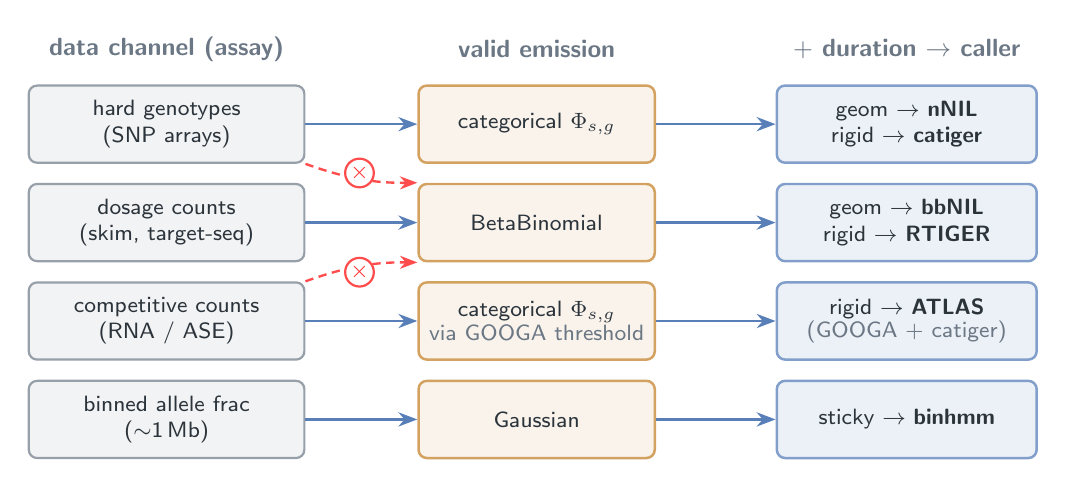
\begin{tikzpicture}[font=\sffamily]

% (figure title + explanatory text live in the LaTeX caption, not in the graphic)
\tikzset{
  chbox/.style={rounded corners=3pt, draw=softgray!70, fill=softgray!9, line width=0.8pt,
                minimum width=3.5cm, minimum height=0.98cm, align=center, font=\footnotesize, text=ink},
  embox/.style={rounded corners=3pt, draw=emitoch!70, fill=emitoch!9, line width=0.9pt,
                minimum width=3.0cm, minimum height=0.98cm, align=center, font=\footnotesize, text=ink},
  cabox/.style={rounded corners=3pt, draw=stateblue!60, fill=stateblue!9, line width=0.9pt,
                minimum width=3.3cm, minimum height=0.98cm, align=center, font=\footnotesize, text=ink},
  flow/.style={-{Stealth[length=2.4mm]}, line width=0.9pt, draw=stateblue!80},
  badflow/.style={-{Stealth[length=2.2mm]}, line width=0.85pt, draw=red!70, dash pattern=on 3pt off 2pt},
  colhead/.style={font=\small\bfseries, text=softgray}}

% column headers
\node[colhead] at (2.6,-1.05) {data channel (assay)};
\node[colhead] at (7.3,-1.05) {valid emission};
\node[colhead] at (12.0,-1.05) {$+$ duration $\to$ caller};

% row 1: hard genotypes -> categorical -> nNIL / catiger
\node[chbox] (ch1) at (2.6,-2.0) {hard genotypes\\(SNP arrays)};
\node[embox] (em1) at (7.3,-2.0) {categorical $\Phi_{s,g}$};
\node[cabox] (ca1) at (12.0,-2.0) {geom $\to$ \textbf{nNIL}\\rigid $\to$ \textbf{catiger}};
\draw[flow] (ch1) -- (em1);   \draw[flow] (em1) -- (ca1);

% row 2: dosage counts -> BetaBinomial -> bbNIL / RTIGER
\node[chbox] (ch2) at (2.6,-3.25) {dosage counts\\(skim, target-seq)};
\node[embox] (em2) at (7.3,-3.25) {BetaBinomial};
\node[cabox] (ca2) at (12.0,-3.25) {geom $\to$ \textbf{bbNIL}\\rigid $\to$ \textbf{RTIGER}};
\draw[flow] (ch2) -- (em2);   \draw[flow] (em2) -- (ca2);

% row 3: competitive / ASE -> (ATLAS threshold) categorical -> nNIL / catiger
\node[chbox] (ch3) at (2.6,-4.5) {competitive counts\\(RNA / ASE)};
\node[embox] (em3) at (7.3,-4.5) {categorical $\Phi_{s,g}$\\[-1pt]{\footnotesize\color{softgray}via GOOGA threshold}};
\node[cabox] (ca3) at (12.0,-4.5) {rigid $\to$ \textbf{ATLAS}\\[-1pt]{\footnotesize\color{softgray}(GOOGA $+$ catiger)}};
\draw[flow] (ch3) -- (em3);
\draw[flow] (em3) -- (ca3);

% row 4: binned -> Gaussian -> binhmm
\node[chbox] (ch4) at (2.6,-5.75) {binned allele frac\\($\sim$1\,Mb)};
\node[embox] (em4) at (7.3,-5.75) {Gaussian};
\node[cabox] (ca4) at (12.0,-5.75) {sticky $\to$ \textbf{binhmm}};
\draw[flow] (ch4) -- (em4);   \draw[flow] (em4) -- (ca4);

% two easily-misused routes (red, marked with X): feeding BetaBinomial data it cannot model
\draw[badflow] (ch1.south east) to[bend right=10] (em2.north west);
\draw[badflow] (ch3.north east) to[bend left=10]  (em2.south west);
\node[circle, fill=white, draw=red!70, line width=0.8pt, inner sep=0.6pt,
      font=\footnotesize\bfseries, text=red!80] at (5.05,-2.62) {$\times$};
\node[circle, fill=white, draw=red!70, line width=0.8pt, inner sep=0.6pt,
      font=\footnotesize\bfseries, text=red!80] at (5.05,-3.88) {$\times$};

\end{tikzpicture}
\end{document}
